
\begin{center}
	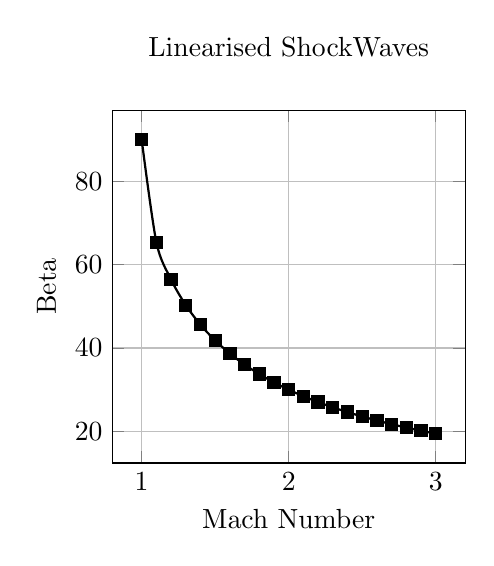
\begin{tikzpicture}
	  \begin{axis}[
		width=0.5\textwidth,
		height=0.5\textwidth,
		xlabel={Mach Number},
		ylabel={Beta},
		title={Linearised ShockWaves},
		title style={yshift=10pt},
		grid=major,
		legend style={legend pos=north west},
		% scaled x ticks=false,  % éventuellement pour afficher en pleine valeur
	  ]
		\addplot[
		  smooth,
		  mark=square*,
		  thick,
		] coordinates {
			(1, 90)
			(1.1, 65.38002267)
			(1.2, 56.44269024)
			(1.3, 50.28486277)
			(1.4, 45.5846914)
			(1.5, 41.8103149)
			(1.6, 38.68218745)
			(1.7, 36.03187907)
			(1.8, 33.7489886)
			(1.9, 31.75686386)
			(2, 30)
			(2.1, 28.43689015)
			(2.2, 27.03569179)
			(2.3, 25.77146174)
			(2.4, 24.62431835)
			(2.5, 23.57817848)
			(2.6, 22.61986495)
			(2.7, 21.73846079)
			(2.8, 20.92483243)
			(2.9, 20.17127135)
			(3, 19.47122063)			
		};	
	  \end{axis}
	\end{tikzpicture}
\end{center}